%------------------------------------------------------------------------------
% Author(s):
% Varaun Ramgoolie
%
% Copyright:
%  Copyright (C) 2020 Brad Bachu, Arjun Mohammed, Varaun Ramgoolie, Nicholas Sammy
%
%  This file is part of Applied-Mathematics-Unit2 and is distributed under the
%  terms of the MIT License. See the LICENSE file for details.
%
%  Description:
%     Year: 2013
%     Module: 3
%     Question: 5
%------------------------------------------------------------------------------

%------------------------------------------------------------------------------
% 5 a
%------------------------------------------------------------------------------

\begin{subquestions}
	
\subquestion
We are given a uniform rod hinged at a point, which is suspended in a horizontal position by a string.

\begin{subsubquestions}

\subsubquestion
	
\textbf{\textit{Simplify and Diagram:}} \\ \\
\begin{figure}[H]
	\begin{center}
		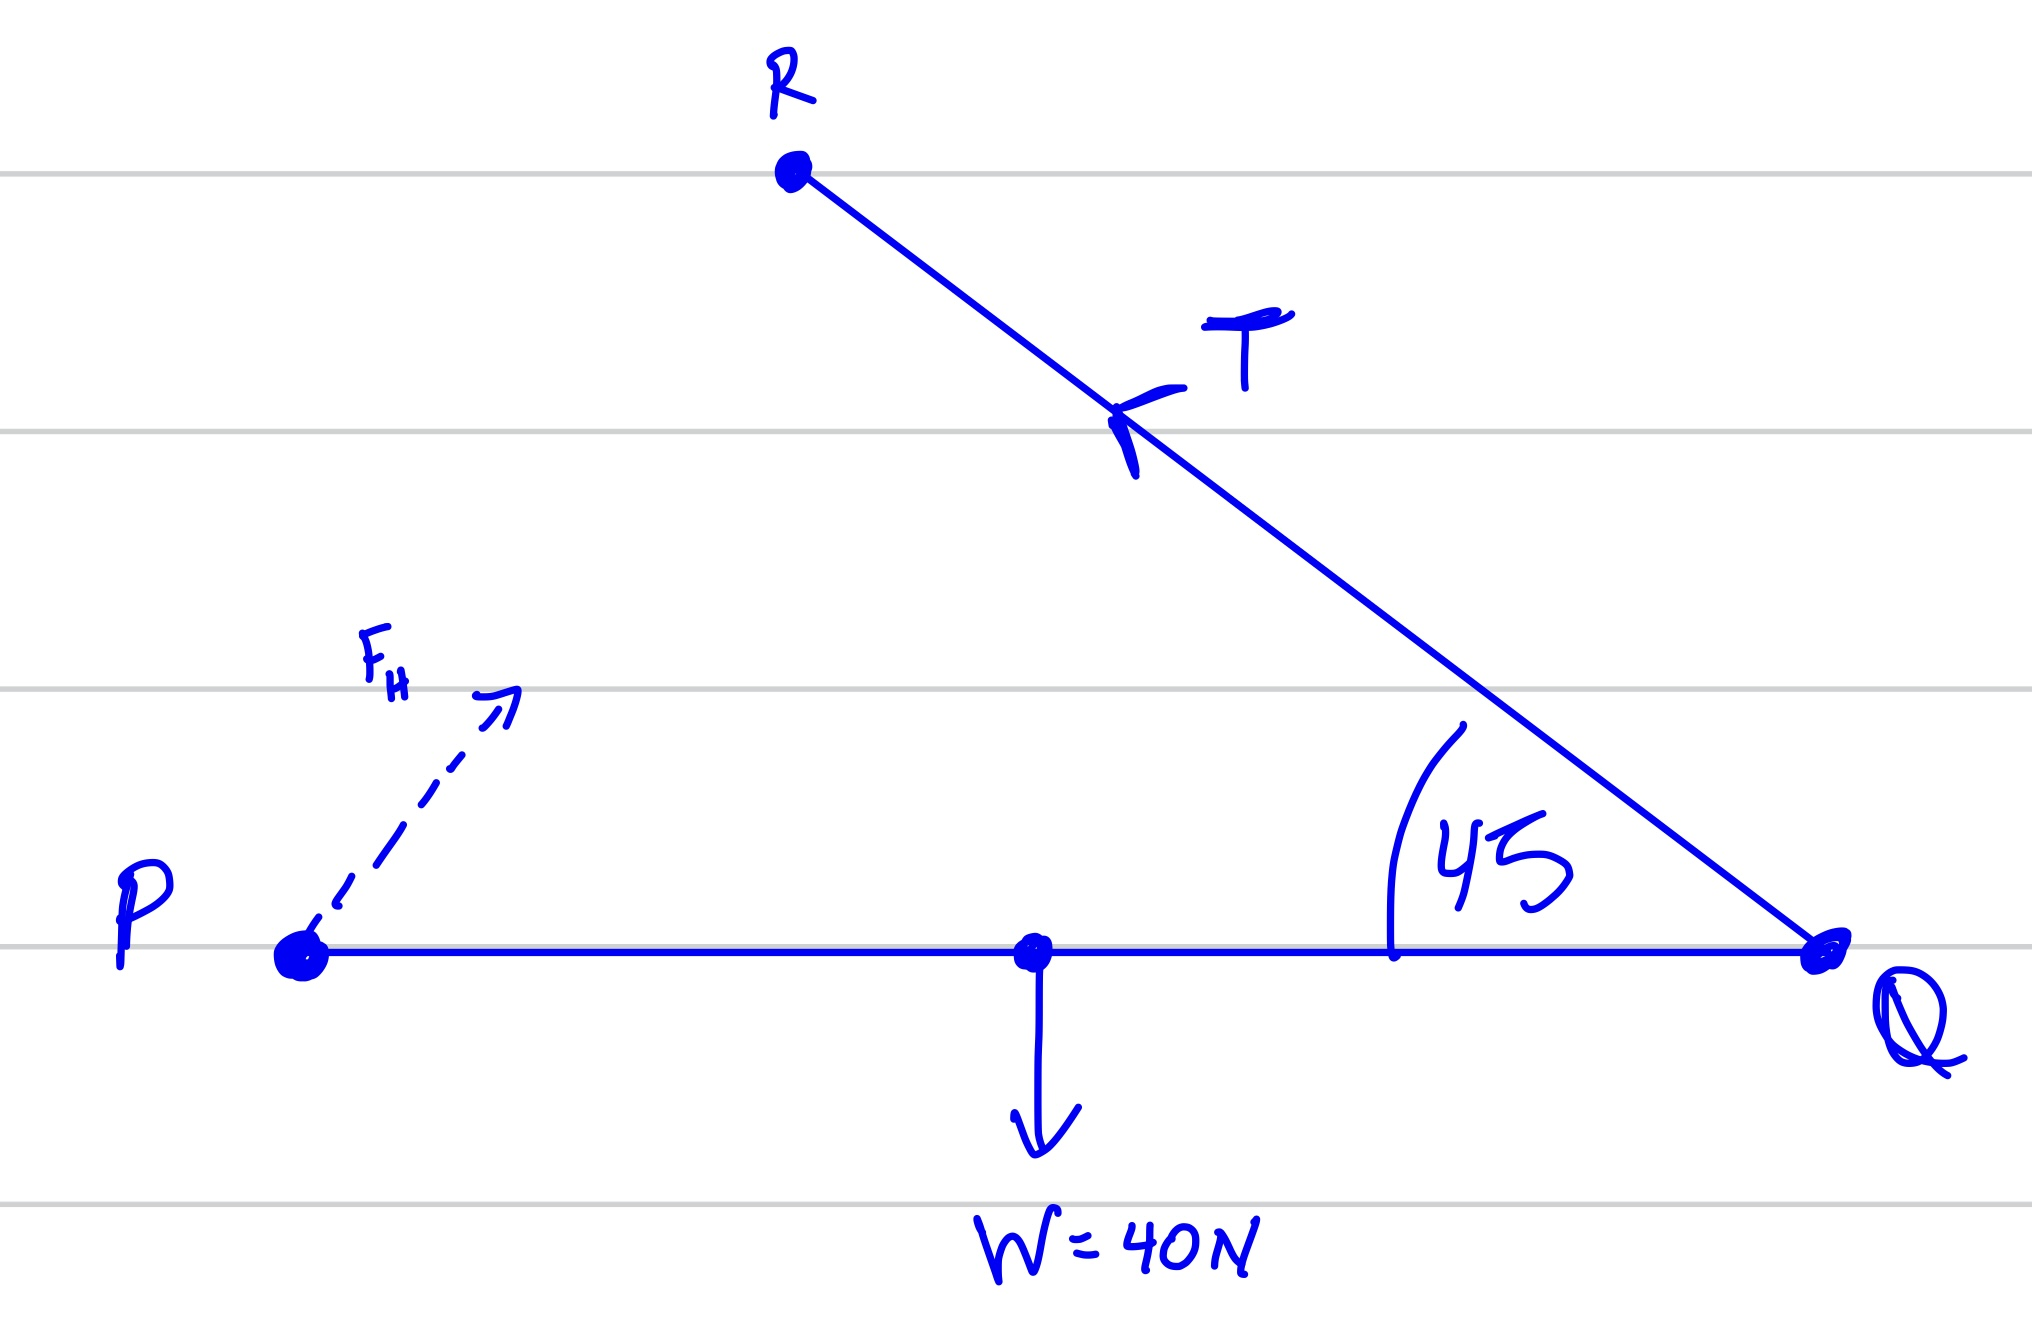
\includegraphics[scale=0.25]{../2013/figures/2013q5-1}
		\caption{\label{2013:q5:Diagram1} Co-planar Force diagram.}
	\end{center}
\end{figure}

%------------------------------------------------------------------------------

\subsubquestion

\textbf{\textit{Simplify and Diagram:}} \\ \\
We can consider \rfig{2013:q5:Diagram1}. We want to find the tension on the string. Let us define,
\begin{itemize}
	\item $\vec{W}$ as the weight of the rod acting at the centre of gravity of the rod,
	\item $\vec{T}$ as that tension on the string acting from Q to R,
	\item $\vec{F_H}$ as the force acting from P to the hinge.  
\end{itemize}
Let us define the length of the rod as $d$. As we are given that the rod is held in equilibrium, we can consider all the forces on PQ and take moments about the point P.




\textbf{\textit{Represent Mathematically:}} \\ \\
We know that the moment of a force is,
\begin{equation}
	\text{Moment} = \text{F} \times \text{$\perp$ distance from pivot} \,.
\end{equation}

We must first resolve the tension in the string as,
\begin{equation}
	\vec{T} = -|T|\cos(45)\xhat + |T|\sin(45)\yhat \,.
\end{equation}

As the body is in equilibrium, we know that the sum of the moments at any point on the rod is 0.




\textbf{\textit{Solve and Evaluate:}}
Taking moments about the point P\footnote{We must only consider the $y$ component of the tension as the $x$ component will not produce a turning force (as it acts in in the direction of PQ).}, we get that,
\begin{align}
	\sum \text{Moments} = (\vec{F_H}\times 0) + (\vec{W} \times \frac{d}{2}) + (|T|\sin(45) \times d) & = 0 \nn \\
	                                             (-|W| \times \frac{d}{2}) + (|T|\sin(45) \times d) & = 0 \nn \\
	                                                                |T|\sin(45) \times d & = |W| \times \frac{d}{2} \nn \\
	                                                                \implies |T| & = \frac{|W|\sqrt{2}}{2} \nn \\
	                                                                             & = \frac{40}{\sqrt{2}}N \,. 
\end{align}

\end{subsubquestions}

%------------------------------------------------------------------------------
% 5 b
%------------------------------------------------------------------------------

\subquestion

\textbf{\textit{Sketch and Translate:}} \\ \\
\begin{figure}[H]
	\begin{center}
		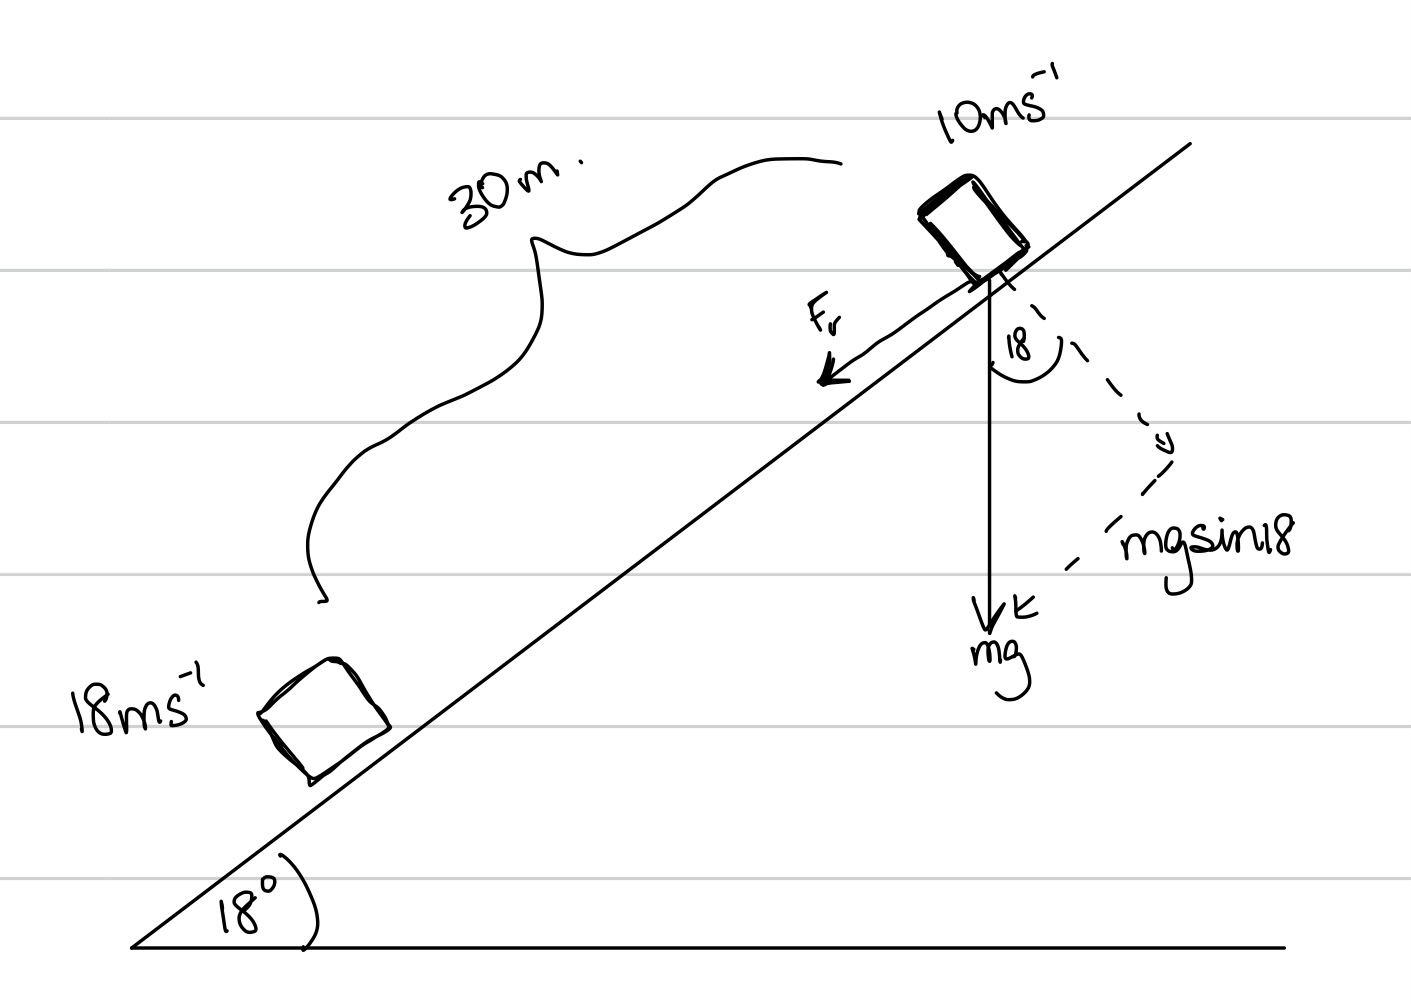
\includegraphics[scale=0.25]{../2013/figures/2013q5-2}
		\caption{\label{2013:q5:Sketch2} Carriage moving up plane.}
	\end{center}
\end{figure}
We are given a carriage which ascends a plane and loses speed on its ascent. As we want to find the frictional resistance, we should begin thinking about what we know about the forces on the carriage and how we can manipulate this information.




\textbf{\textit{Simplify and Diagram:}} \\ \\
\begin{figure}[H]
	\begin{center}
		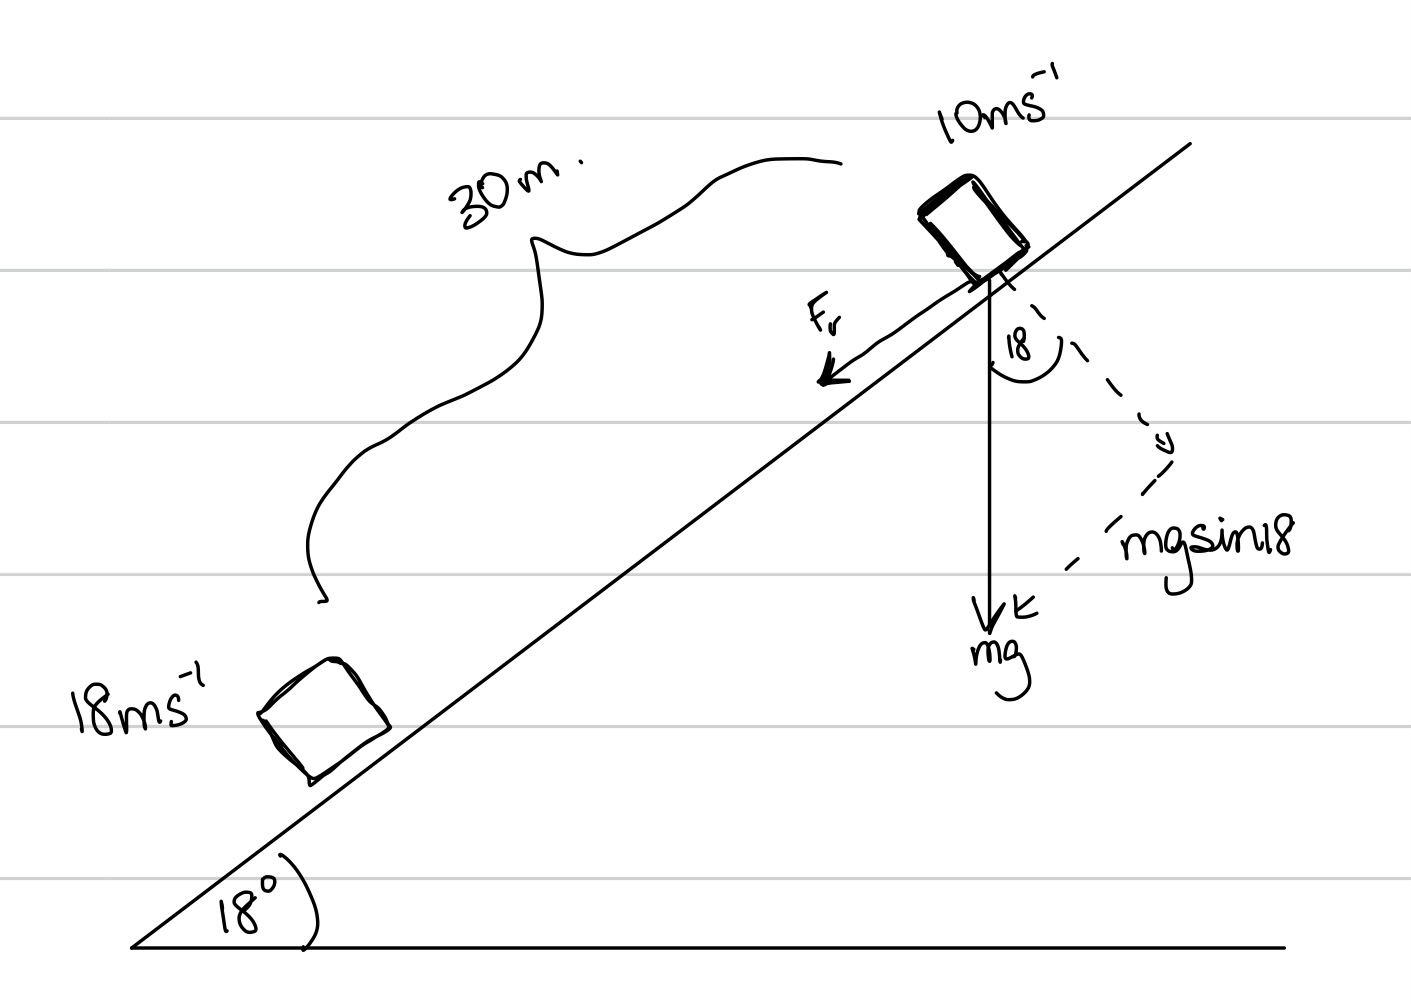
\includegraphics[scale=0.25]{../2013/figures/2013q5-2}
		\caption{\label{2013:q5:Diagram2} Carriage moving up plane.}
	\end{center}
\end{figure}
We will first assume that the carriage behaves as a point particle. Let us define,
\begin{itemize}
	\item $\vec{F_f}$ as the frictional force opposing motion,
	\item $\vec{W}$ as the weight of the carriage,
	\item $\vec{R}$ as the normal reaction force on the plane.
\end{itemize}
Using the velocities that we  are given, we can find the deceleration of the body. Using Newton's Second Law, we can find the relationship between the acceleration and the resultant force on the body and then we can solve for our frictional force.




\textbf{\textit{Represent Mathematically:}} \\ \\
From the information that we are given, we can find the acceleration of the body using,
\begin{align}
	v^2 & = u^2 + 2as \nn \\
	\implies a & = \frac{v^2-u^2}{2s} \,. \label{2013:q5:AEqn1}
\end{align}

Let us resolve the weight of the carriage as,
\begin{equation}
	\vec{W} = -|W|\sin(18)\xhat-|W|\cos(18)\yhat \,.
\end{equation}

Let us resolve the frictional force as,\footnote{We have used the magnitude of $\vec{F_f}$ and $F_f$.}
\begin{equation}
	\vec{F_f} = -F_f \xhat
\end{equation}

From Newton's Second law, we get that the resultant force, $F_R$, in the $x$ direction is,
\begin{equation}
	F_R = \sum F \xhat = ma \,.	\label{2013:q5:Newton1}
\end{equation}




\textbf{\textit{Solve and Evaluate:}} \\ \\
Using \req{2013:q5:AEqn1}, we get that,
\begin{align}
	a & = \frac{v^2-u^2}{2s} \nn \\
	  & = \frac{10^2-18^2}{2(30)} \nn \\
	  & = \frac{-224}{60} = \frac{-56}{15} \,. 
\end{align}

Using \req{2013:q5:Newton1}, we can now find,
\begin{align}
	F_R = \sum F \xhat & = ma \nn \\
	      -|W|\sin(18) - F_f & = (700)(\frac{-56}{15}) \nn \\
	      \implies F_f & = -(700)(\frac{-56}{15})-|W|\sin(18) \nn \\
	                   & = 2613.3-mg\sin(18) \nn \\
	                   & = 2613.3-(700)(10)\sin(18) \nn \\
	                   & = 450.18N
\end{align}

\TODO{I dont understand how to do the energy method. Can i Calculate work against gravity AND force against friction if theyre both not perpendicular to each other?}

%------------------------------------------------------------------------------
% 5 c
%------------------------------------------------------------------------------

\subquestion
We are given a scenario where a cyclist gradually climbs a hill. Their velocity is given as a differential equation.

\begin{subsubquestions}
	
\subsubquestion

\textbf{\textit{Sketch and Translate:}} \\ \\
\begin{figure}[H]
	\begin{center}
		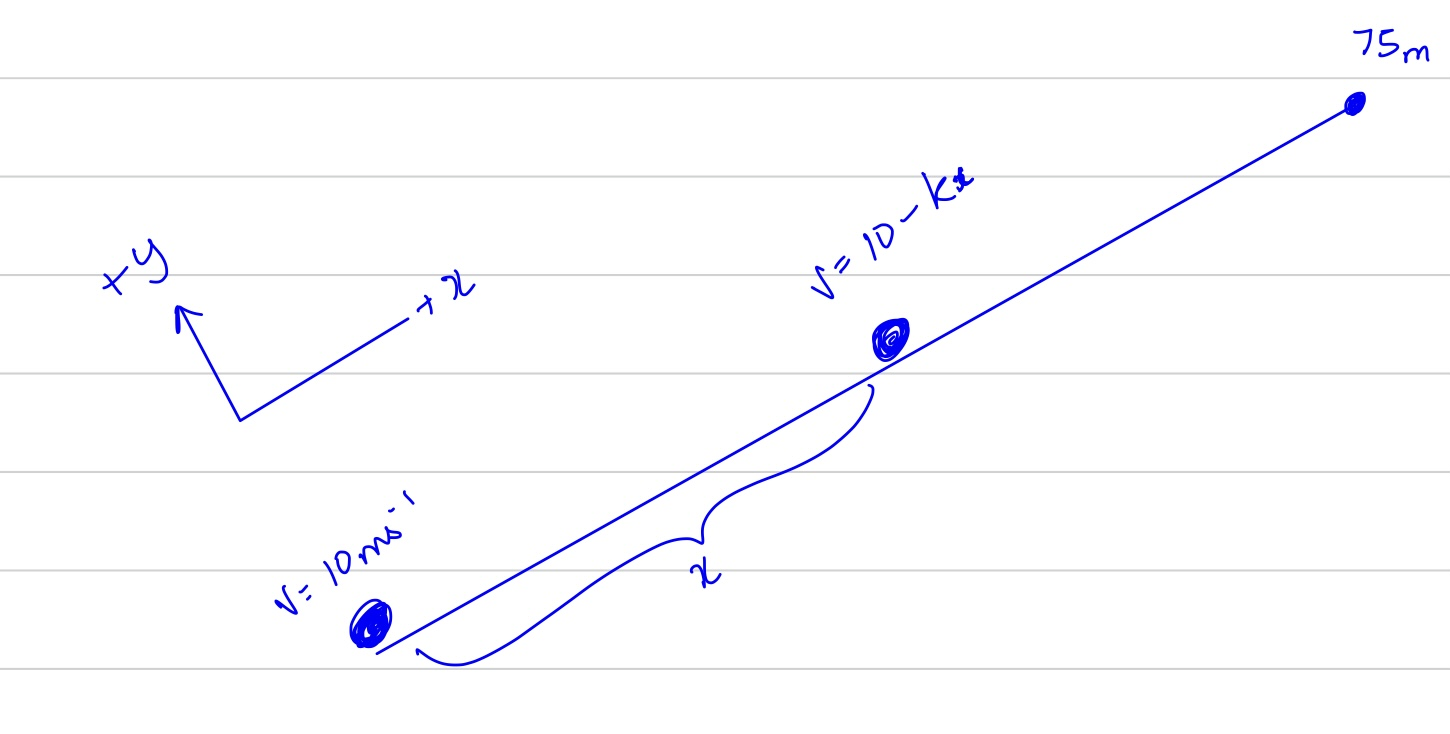
\includegraphics[scale=0.25]{../2013/figures/2013q5-3}
		\caption{\label{2013:q5:Sketch3} Cyclist climbing hill.}
	\end{center}
\end{figure}
As we are given the approach velocity of the cyclist (before they begin the ascent), we can think about how this might be helpful (if at all) to solve out differential equation.
	
	
	
	
\textbf{\textit{Simplify and Diagram:}} \\ \\
\begin{figure}[H]
	\begin{center}
		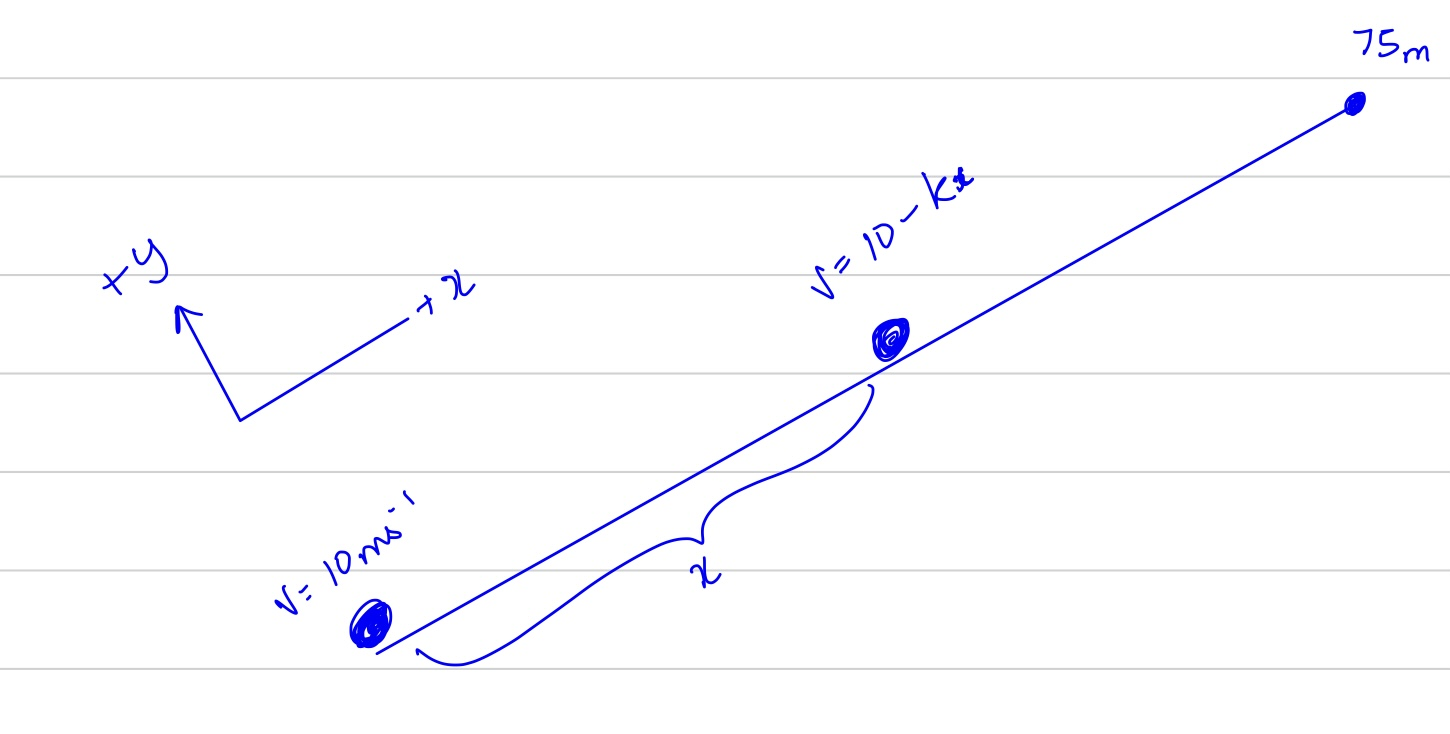
\includegraphics[scale=0.25]{../2013/figures/2013q5-3}
		\caption{\label{2013:q5:Diagram3} Cyclist climbing hill.}
	\end{center}
\end{figure}
We can notice that, from the differential equation given, the velocity decreases linearly as the cyclist travels $x$m. We also should notice that, at $t=0$, the displacement $x=0$.




\textbf{\textit{Represent Mathematically:}} \\ \\
We can separate the variables of the differential equation as follows,
\begin{align}
	\ddd{x}{t} & = 10-kx \nn \\
	\frac{1}{10-kx}\dd x & = \dd t \,.
\end{align}




\textbf{\textit{Solve and Evaluate:}} \\ \\
By using the bounds $(x_1,t_1)=(0,0)$ and $(x_2,t_2)=(x',t')$, we get that,
\begin{align}
	\int_{x_1}^{x_2}\frac{1}{10-kx}\dd x & = \int_{t_1}^{t_2}\dd t \nn \\
	\frac{-1}{k} \int_{0}^{x'}\frac{-k}{10-kx}\dd x & = \int_{0}^{t'}\dd t \nn \\
	\frac{-1}{k} \left[\ln(10-kx)\right]_0^{x'} & = \left[t\right]_0^{t'} \nn \\
	\frac{-1}{k} \left[\ln(10-kx')-\ln(10)\right] & = t' \nn \\
	\frac{1}{k} \left[\ln(10)-\ln(10-kx')\right] & = t' \nn \\
	\implies \frac{1}{k} \ln\left(\frac{10}{10-kx'}\right) & = t' \,.
\end{align}

%------------------------------------------------------------------------------

\subsubquestion

\textbf{\textit{Simplify and Diagram:}} \\ \\
We can use \rfig{2013:q5:Diagram3}. As we are given $\frac{\dd x}{\dd t}$, by definition, we have an equation for the velocity of the cyclist. We can therefore substitute our values and solve for $k$.




\textbf{\textit{Represent Mathematically:}} \\ \\
By definition, we have,
\begin{equation}
	v = 10-kx \,.
\end{equation}




\textbf{\textit{Solve and Evaluate:}} \\ \\
By substituting $v=4$ms$^{-1}$ and $x=75$m, we get that,
\begin{align}
	4 & = 10-75k \nn \\
	\implies k & = \frac{6}{75} \,.
\end{align}

\end{subsubquestions}

\end{subquestions}